\documentclass[11pt]{article}
\usepackage[margin=1in]{geometry}
\usepackage{tikz}
\usetikzlibrary{shapes,arrows,positioning,calc}
\usepackage{graphicx}
\usepackage{amsmath}
\usepackage{enumitem}
\usepackage{booktabs}
\usepackage[hidelinks]{hyperref}

\setlist{nosep,leftmargin=*}

\title{\vspace{-1.5em}\textbf{Sigil: Universal Hand Gesture Control Framework for Command-Controllable Environments}\vspace{-0.5em}}
\author{
  Prathamesh Sankhe (231080061) \\
  Yadnyesh Patil (231080050) \\
  Advait Desai (241080902) \\
  Raj Kharwal (231080052)
}
\date{April 2026}

\begin{document}
\maketitle
\vspace{-1em}

\section{Problem Statement}

Modern workflows across diverse environments—from desktop computing to presentations and virtual collaboration—remain heavily dependent on keyboard and mouse input. This creates friction in scenarios where hands-free control would enhance productivity:

\begin{itemize}
\item \textbf{Presentations \& Teaching}: Instructors need to control slides and multimedia while maintaining audience engagement
\item \textbf{Virtual Meetings}: Professionals require quick access to mute, reactions, and screen sharing controls
\item \textbf{Desktop Management}: Linux users running tiling window managers lack intuitive gesture interfaces
\item \textbf{Media Production}: Content creators need hands-free playback and timeline control
\end{itemize}

Existing gesture control solutions suffer from: \textbf{hardware barriers} (require expensive depth cameras $>$\$200), \textbf{platform limitations} (mobile-only or proprietary systems), \textbf{performance issues} (high latency $>$150ms, CPU usage $>$50\%), and \textbf{limited customization} (no user training capabilities).

\textbf{Core Challenge:} Develop a universal gesture control framework enabling sub-80ms latency, $\geq$80\% accuracy using only standard webcam, with $<$25\% CPU overhead, adaptable to any command-controllable environment through keyboard shortcuts, shell commands, or APIs.

\section{Objective}

\subsection{Primary Goal}

Develop a universal hand gesture control framework that enables users to record, train, and map custom hand gestures (instant, gradual, sequential) to any command-controllable environment—presentations, virtual meetings, window managers, and media applications—with performance suitable for daily use.

\subsection{Target Environments \& Key Objectives}

\textbf{Environments:} Window Managers (Hyprland, Sway, i3), Presentations (Impress, Slides, PowerPoint), Virtual Meetings (Zoom, Meet, Teams), Media Players (VLC, MPV, OBS)

\textbf{Performance:} Latency $<$80ms, 30-60 fps tracking, CPU $<$25\%, inference $<$30ms

\textbf{Accuracy:} Landmark detection $\geq$95\%, gesture classification $\geq$80\%, zero false positives

\textbf{Gesture Types:} Instant (peace sign $\rightarrow$ keyboard shortcuts), Gradual (pinch openness $\rightarrow$ volume control), Sequential (swipe patterns $\rightarrow$ command chains)

\textbf{Universal Compatibility:} xdotool/ydotool (keyboard), shell commands, window manager IPC (hyprctl/swaymsg/i3-msg), D-Bus/MPRIS (media control), profile auto-switching

\section{Methodology}

\subsection{Architecture Overview}

\begin{figure}[h]
\centering
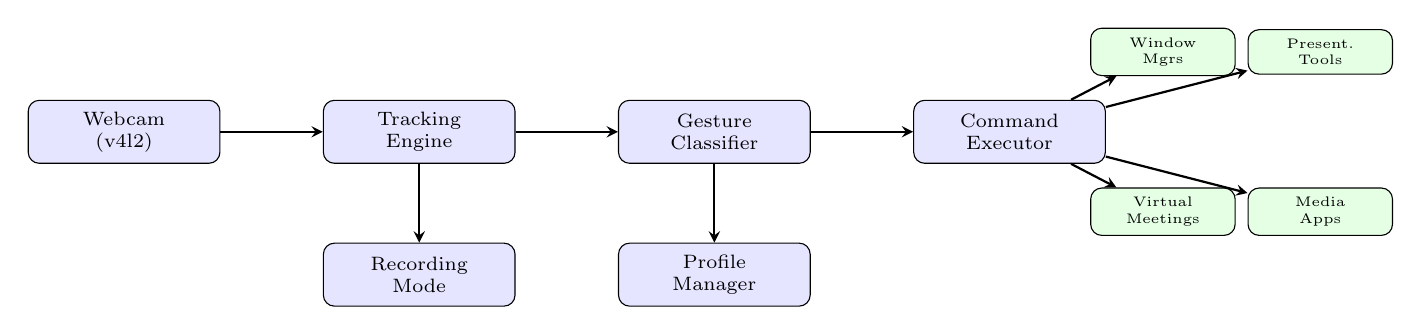
\begin{tikzpicture}[
  node distance=1.3cm,
  block/.style={rectangle, draw, fill=blue!10, text width=2.2cm, text centered, rounded corners, minimum height=0.8cm, font=\scriptsize},
  appblock/.style={rectangle, draw, fill=green!10, text width=1.6cm, text centered, rounded corners, minimum height=0.5cm, font=\tiny},
  arrow/.style={->, >=stealth, thick}
]
  \node[block] (webcam) {Webcam\\(v4l2)};
  \node[block, right=of webcam] (track) {Tracking\\Engine};
  \node[block, right=of track] (gesture) {Gesture\\Classifier};
  \node[block, right=of gesture] (executor) {Command\\Executor};
  
  \node[appblock, above right=0.3cm and -0.2cm of executor] (wm) {Window\\Mgrs};
  \node[appblock, right=0.15cm of wm] (pres) {Present.\\Tools};
  \node[appblock, below right=0.3cm and -0.2cm of executor] (vc) {Virtual\\Meetings};
  \node[appblock, right=0.15cm of vc] (media) {Media\\Apps};
  
  \node[block, below=1cm of track] (record) {Recording\\Mode};
  \node[block, below=1cm of gesture] (config) {Profile\\Manager};
  
  \draw[arrow] (webcam) -- (track);
  \draw[arrow] (track) -- (gesture);
  \draw[arrow] (gesture) -- (executor);
  \draw[arrow] (executor) -- (wm);
  \draw[arrow] (executor) -- (pres);
  \draw[arrow] (executor) -- (vc);
  \draw[arrow] (executor) -- (media);
  \draw[arrow] (track) -- (record);
  \draw[arrow] (gesture) -- (config);
\end{tikzpicture}
\caption{Universal System Architecture}
\end{figure}

\subsection{Phase 1: Tracking Engine}

MediaPipe Hand Landmarker extracts \textbf{21 3D landmarks per hand} + handedness. Configuration: \texttt{num\_hands=2}, \texttt{min\_detection\_confidence=0.7}, \texttt{running\_mode=VIDEO}. Input: standard webcam $\geq$720p via v4l2/pipewire. Fallback to legacy \texttt{mp\_hands} if API changes.

\subsection{Phase 2: Gesture Classification}

\textbf{Feature Engineering:} 101-dimensional vector (normalized 3D positions, finger curl states, inter-landmark distances, joint angles, palm orientation, finger spread)

\textbf{Models:} Instant (MediaPipe Gesture Recognizer .tflite or scikit-learn MLP/KNN), Gradual (geometric features: pinch strength, hand openness), Sequential (time-series buffering 8-30 frames with DTW or LSTM)

\subsection{Phase 3: Recording \& Training}

\textbf{Trigger:} Hotkey \texttt{Super+Alt+G}. Collect 50-200 samples per gesture class. Storage: \texttt{\textasciitilde/.local/share/sigil/recordings/}. Training: \texttt{sigil train --type instant --class <name>} exports to .tflite model.

\subsection{Phase 4: Profile System \& Execution}

\textbf{Profiles:} desktop.yaml (window controls), presentation.yaml (slides), meeting.yaml (mute/reactions), media.yaml (playback). Auto-switching detects active application.

\textbf{Configuration Examples:}

\begin{verbatim}
# presentation.yaml
gestures:
  - name: "next_slide"
    action: "xdotool key Right"
  - name: "previous_slide"
    action: "xdotool key Left"

# meeting.yaml
gestures:
  - name: "toggle_mute"
    action: "xdotool key alt+a"
  - name: "raise_hand"
    action: "xdotool key alt+y"

# desktop.yaml
gestures:
  - name: "close_window"
    action: "hyprctl dispatch killactive"
  - name: "next_workspace"
    action: "hyprctl dispatch workspace +1"
\end{verbatim}

\textbf{Runtime Loop:} Capture frame $\rightarrow$ Detect hands (21 landmarks × 2) $\rightarrow$ Classify with confidence $\rightarrow$ Temporal smoothing (9-frame buffer, 2-frame confirmation) $\rightarrow$ Match profile mappings $\rightarrow$ Execute command (keyboard/shell/IPC/D-Bus) $\rightarrow$ Blanking period (1000ms cooldown)

\subsection{Phase 5: Optimization}

Model compression ($<$30ms inference), multi-threading (capture/inference/execution), auto-tuning FPS (30$\rightarrow$15 fps fallback based on CPU), logging (debug/info/error to journalctl).

\subsection{Technology Stack \& Timeline}

\begin{table}[h]
\centering
\small
\begin{tabular}{@{}ll@{}}
\toprule
\textbf{Component} & \textbf{Technology} \\
\midrule
Hand tracking & MediaPipe $\geq$0.10.14 \\
Classifier & Model Maker .tflite / scikit-learn \\
Camera I/O & OpenCV $\geq$4.9 \\
Config & PyYAML $\geq$6.0 \\
Keyboard sim & xdotool/ydotool \\
Platform & Linux (X11/Wayland) \\
Hardware & Webcam $\geq$720p, AVX2 CPU \\
\bottomrule
\end{tabular}
\caption{Technology Stack}
\end{table}

\begin{table}[h]
\centering
\small
\begin{tabular}{@{}lc@{}}
\toprule
\textbf{Milestone} & \textbf{Duration} \\
\midrule
M1: Tracking + visualization & 1-2 weeks \\
M2: Instant gesture recognition & 2-3 weeks \\
M3: Gradual + sequential & 2-3 weeks \\
M4: Profile system + integration & 1-2 weeks \\
M5: Optimization + packaging & 1-2 weeks \\
\midrule
\textbf{Total MVP} & \textbf{9-12 weeks} \\
\bottomrule
\end{tabular}
\caption{Development Timeline}
\end{table}

\subsection{Success Criteria}

\textbf{Functional:} Record 3+ gestures (50 samples each), train $<$60s, profile auto-switching works, commands trigger across environments

\textbf{Performance:} Latency $<$80ms, CPU $<$25\%, accuracy $\geq$80\%, zero false positives (5-min idle)

\textbf{Use Cases:}

\begin{table}[h]
\centering
\small
\begin{tabular}{@{}lll@{}}
\toprule
\textbf{Environment} & \textbf{Gesture} & \textbf{Action} \\
\midrule
Presentation & Right swipe & Next slide \\
Meeting & Peace sign & Toggle mute \\
Desktop & Close fist & Close window \\
Media & Thumbs right & Play/pause \\
\bottomrule
\end{tabular}
\caption{Multi-Environment Examples}
\end{table}

\vspace{1em}
\noindent\textbf{Repository:} \url{https://github.com/PMS61/sigil}

\noindent\textbf{Primary Focus:} Initial implementation targets Hyprland on CachyOS/Arch as reference, with architecture designed for universal environment support.

\end{document}
